\documentclass{article}
\usepackage[a4paper, margin=3mm, landscape]{geometry}
\usepackage{multicol}
\usepackage{xcolor}
\usepackage{enumitem}
\usepackage{amsmath}
\usepackage{amsfonts}
\usepackage{listings}
\usepackage{soul}
\usepackage{graphicx}

\pdfinfo{
    /Title (ACC1701x.pdf)
    /Creator (TeX)
    /Producer (pdfTeX 1.40.0)
    /Author (Vincent Pang)
    /Subject (CS2106)
    /Keywords (CS2106, nus, cheatsheet, pdf)
}

\graphicspath{ {./img/} }

\pagestyle{empty}
\setcounter{secnumdepth}{0}
\setlength{\columnseprule}{0.25pt}

% Redefine section commands to use less space
\makeatletter
\renewcommand{\section}{\@startsection{section}{1}{0mm}%
    {-1ex plus -.5ex minus -.2ex}%
    {0.5ex plus .2ex}%x
{\normalfont\large\bfseries}}
\renewcommand{\subsection}{\@startsection{subsection}{2}{0mm}%
    {-1explus -.5ex minus -.2ex}%
    {0.5ex plus .2ex}%
{\normalfont\normalsize\bfseries}}
\renewcommand{\subsubsection}{\@startsection{subsubsection}{3}{0mm}%
    {-1ex plus -.5ex minus -.2ex}%
    {1ex plus .2ex}%
{\normalfont\small\bfseries}}%
\makeatother

% Adjust spacing for all itemize/enumerate
\setlength{\leftmargini}{0.5cm}
\setlength{\leftmarginii}{0.5cm}
\setlist[itemize,1]{leftmargin=2mm,labelindent=1mm,labelsep=1mm}
\setlist[itemize,2]{leftmargin=2mm,labelindent=1mm,labelsep=1mm}

% Font
\renewcommand{\familydefault}{\sfdefault}

% Define colors for math formulas
\definecolor{myblue}{cmyk}{1,.72,0,.38}
\everymath\expandafter{\the\everymath \color{myblue}}

% Custom command for keywords
\definecolor{highlight}{RGB}{251,243,218}
\newcommand{\keyword}[2][]{\sethlcolor{highlight}\hl{\textbf{#2}} #1 - }
\newcommand{\ilkeyword}[1]{\sethlcolor{highlight}\hl{\textbf{#1}}}

% Define colors and style for code
\definecolor{codegreen}{rgb}{0,0.6,0}
\definecolor{codegray}{rgb}{0.5,0.5,0.5}
\definecolor{codered}{HTML}{CC241D}
\definecolor{backcolor}{rgb}{0.95,0.95,0.95}
\lstdefinestyle{codestyle}{
    backgroundcolor = \color{backcolor},
    commentstyle = \color{codegray},
    keywordstyle = \color{codered},
    stringstyle = \color{codegreen},
    basicstyle = \ttfamily,
    breakatwhitespace = false,
    showstringspaces = false,
    breaklines = true,
    showtabs = false,
    tabsize = 2
}
\lstset{style = codestyle}

% -----------------------------------------------------------------------
\begin{document}
\begin{multicols*}{3}
\footnotesize

% Title box
\begin{center}
    \fbox{
        \parbox{0.8\linewidth}{
            \centering \textcolor{black}{
                {\Large\textbf{CS2106}} \\
                \normalsize{AY22/23 Sem 2}} \\
                {\footnotesize \textcolor{gray}{github.com/securespider}}
        }
    }
\end{center}
\section{01. Introduction}
\keyword{OS}{Program that acts as an intermediary between user and hardware}

\subsection{Different architectures}
\subsubsection{Harvard architecture}
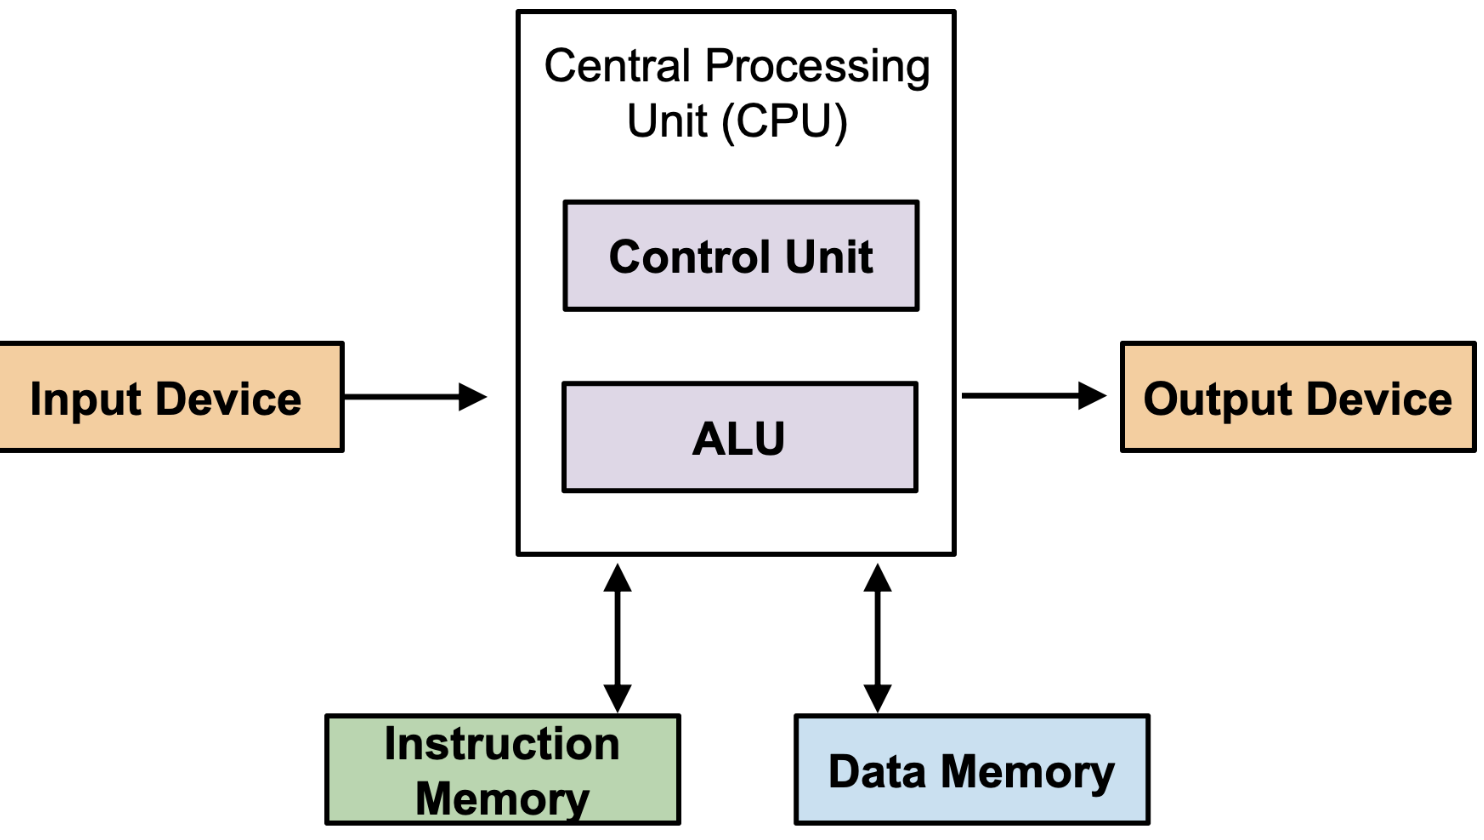
\includegraphics[scale=0.2]{harvard-architecture}
\subsubsection{Von Neumann architecture}
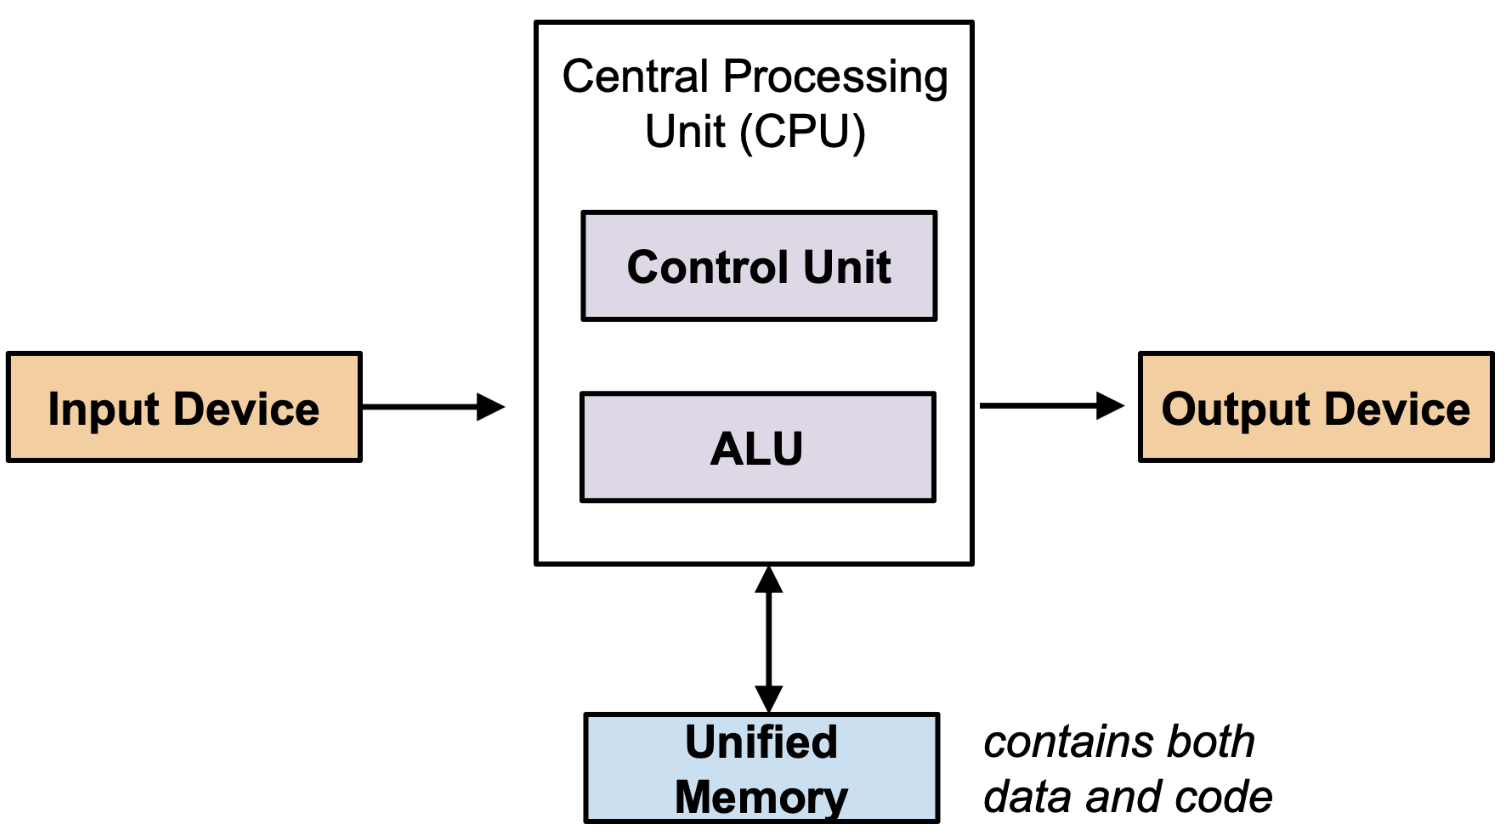
\includegraphics[scale=0.2]{von-neumann}

\begin{description}
	\item[Difference]{Separate vs common storage pathway for code and data}
\end{description}
Why do we need OS?

\subsection{Mainframe}
Old analog "computers" using physical cards for programming
\subsubsection{Improvements}
\begin{itemize}
	\item Problem: Batch processing inefficient
	\item Solution: Multiprogramming
	\begin{itemize}
		\item Loading multiple jobs that runs while other jobs using I/O
		\item Overlapping computation with I/O
	\end{itemize}
	\item Problem: Only one user 
	\item Solution: Time sharing OS
	\begin{itemize}
		\item Multiple concurrent users using terminals
		\item User job scheduling 
		\item Memory management
		\item \keyword{Hardware virtualization}{Each program executes as if it had all resources}
	\end{itemize}
\end{itemize}


\subsection{Motivation}
\begin{enumerate}
	\item Abstraction
	\begin{itemize}
		\item Hide low level details and present common, high-level functionality to users
	\end{itemize}
	\item Resource allocation
	\begin{itemize}
		\item Allow concurrent usage of resource and execute programs simultaneously
		\item Arbitrate conflicting request fairly and efficiently
	\end{itemize}
	\item Control programs
	\begin{itemize}
		\item Restrict resource allocation
		\item Security, protection and error prevention
		\item Ensure proper use of device
	\end{itemize}
\end{enumerate}
\subsubsection{Advantage}
\begin{itemize}
	\item Portable and flexible
	\item Use computer resources efficiently
\end{itemize}
\subsubsection{Disadvantage}
\begin{itemize}
	\item Significant overhead
\end{itemize}

\subsubsection{OS vs User Program}
Similarities
\begin{itemize}
	\item Both softwares
\end{itemize}
Difference
\begin{itemize}
	\item OS runs in \keyword{kernel mode}{Access to all hardware resources}
	\item User programs run in \keyword{User mode}{Limited access}
	\item User programs use syscalls to communicate with OS for hardware processes
\end{itemize}
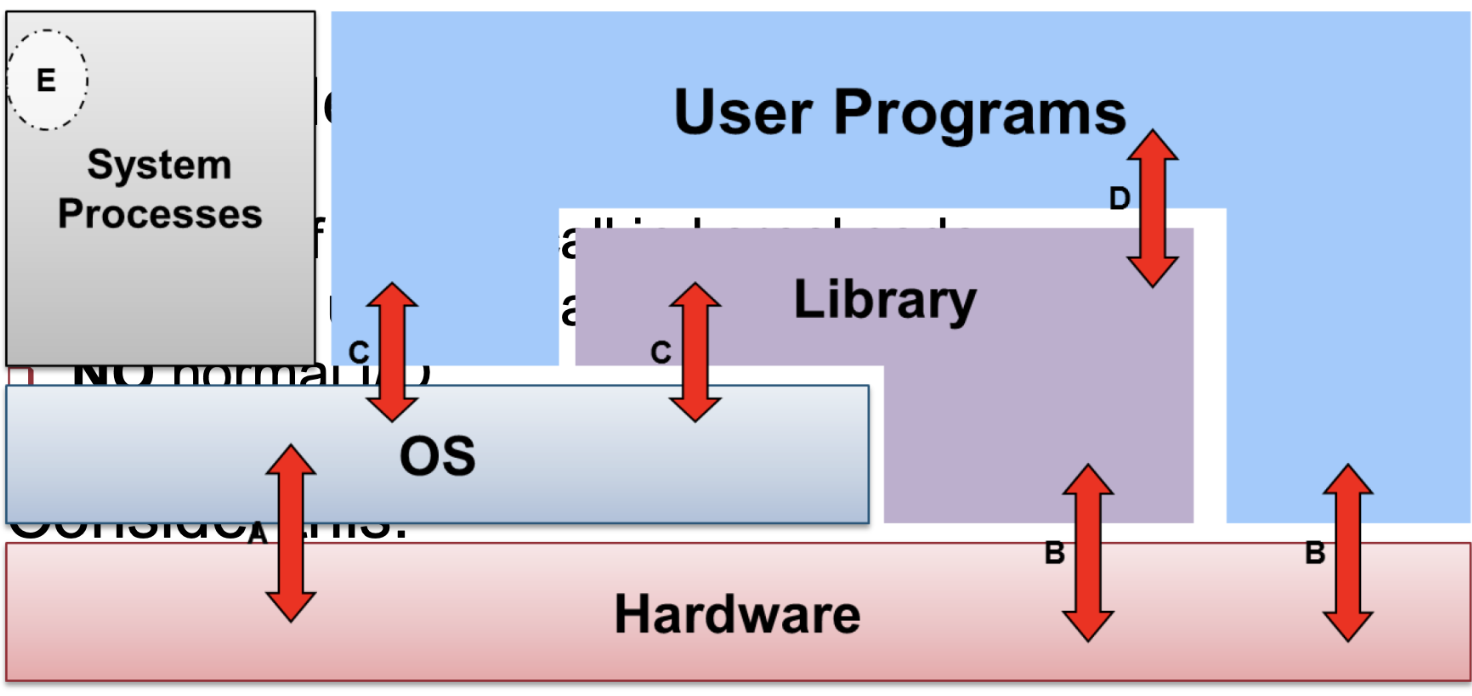
\includegraphics[scale=0.2]{os-interaction}
\\Why OS dont occupy entire hardware layer
\begin{itemize}
	\item Slow to have all operations pass through intermediary
	\item User programs can have direct interaction with hardware (eg. Arithmetic) during low risk operations
\end{itemize}

\subsection{OS structure}
\subsubsection{Monolithic OS}
\begin{itemize}
	\item One big kernel program
	\item Well understood and has good performance
	\item Highly \keyword{coupled}{internal structure interconnected that unintentionally affect each other}
\end{itemize}
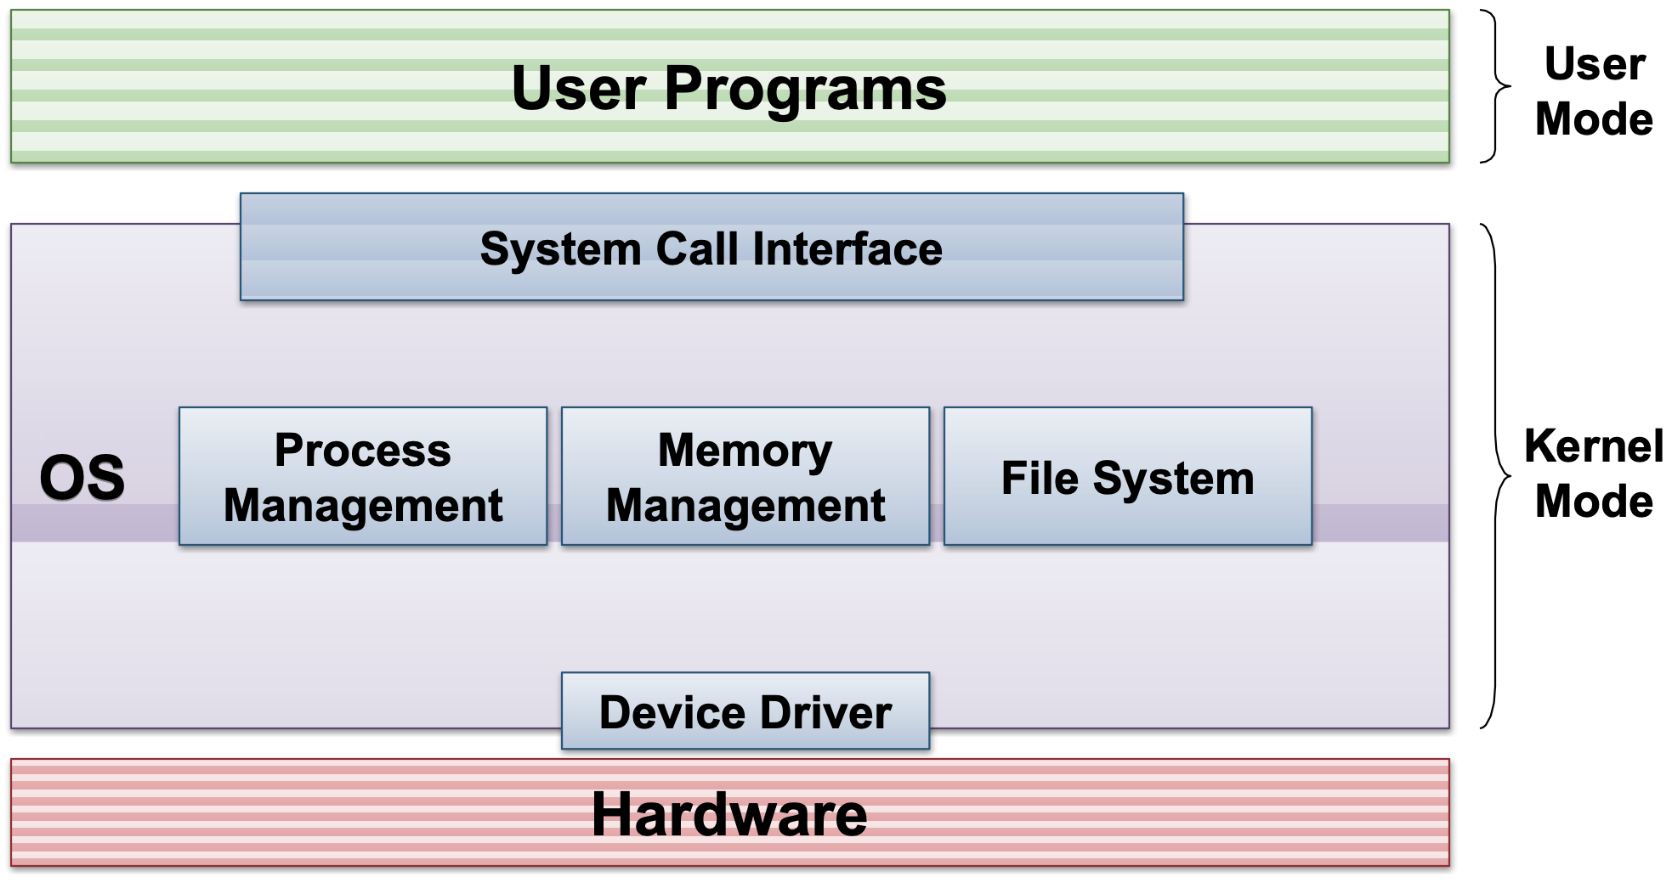
\includegraphics[scale=0.2]{monolithic-os}

\subsubsection{Microkernel}
\begin{itemize}
	\item Small clean
	\item Basic and essential facilities
	\item IPC communication OR run external programs outside OS
	\item Robust and more \keyword{modular}{Extendible and maintainable}
	\item Better isolation btw kernel and services
	\item Lower performance
\end{itemize}
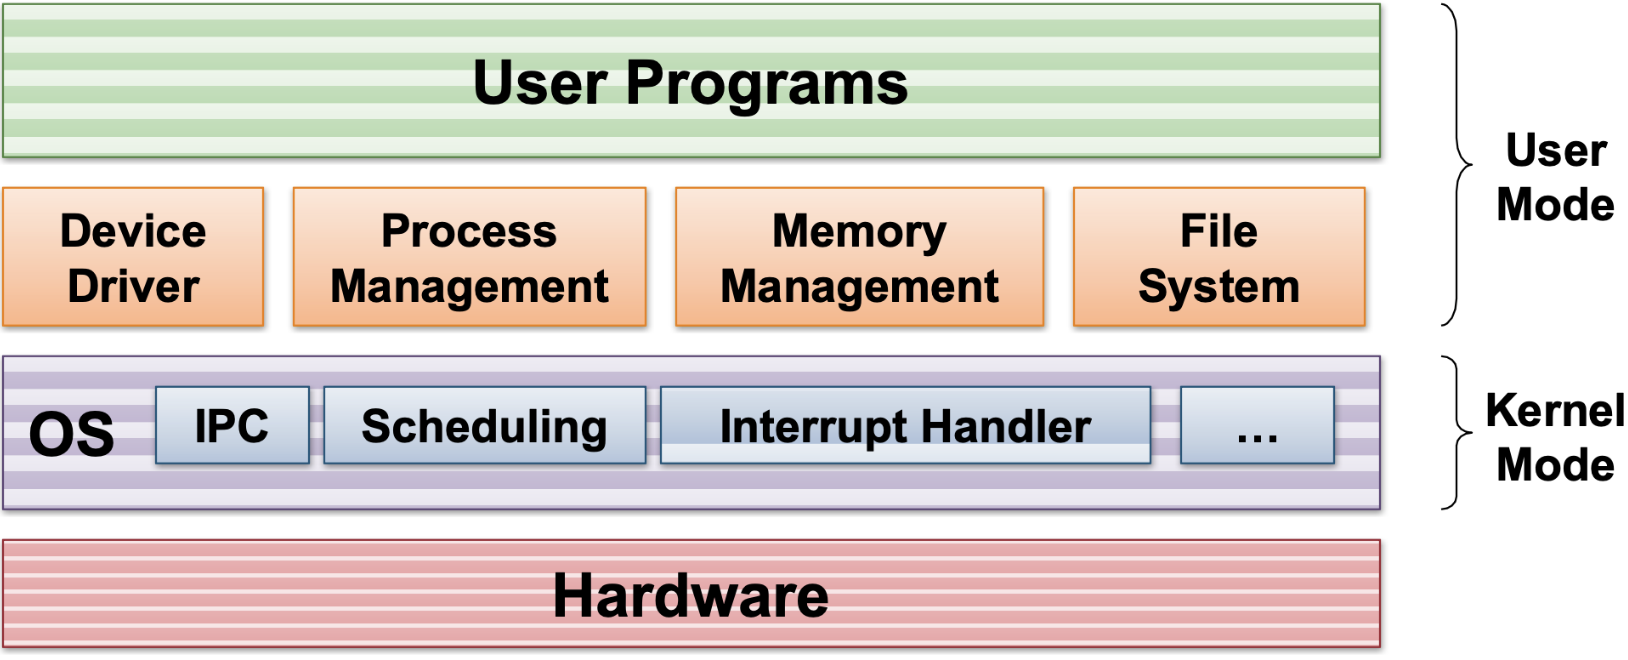
\includegraphics[scale=0.32]{microkernel-os}
%--------------------------------------------------------------------------------------------------------------------

\section{02. Process abstraction}
\subsection{Motivation}
\begin{itemize}
	\item Allow concurrent usage of hardware
	\item Multiple programs sharing the same processors/IO
\end{itemize}

\subsection{Computer organisation}
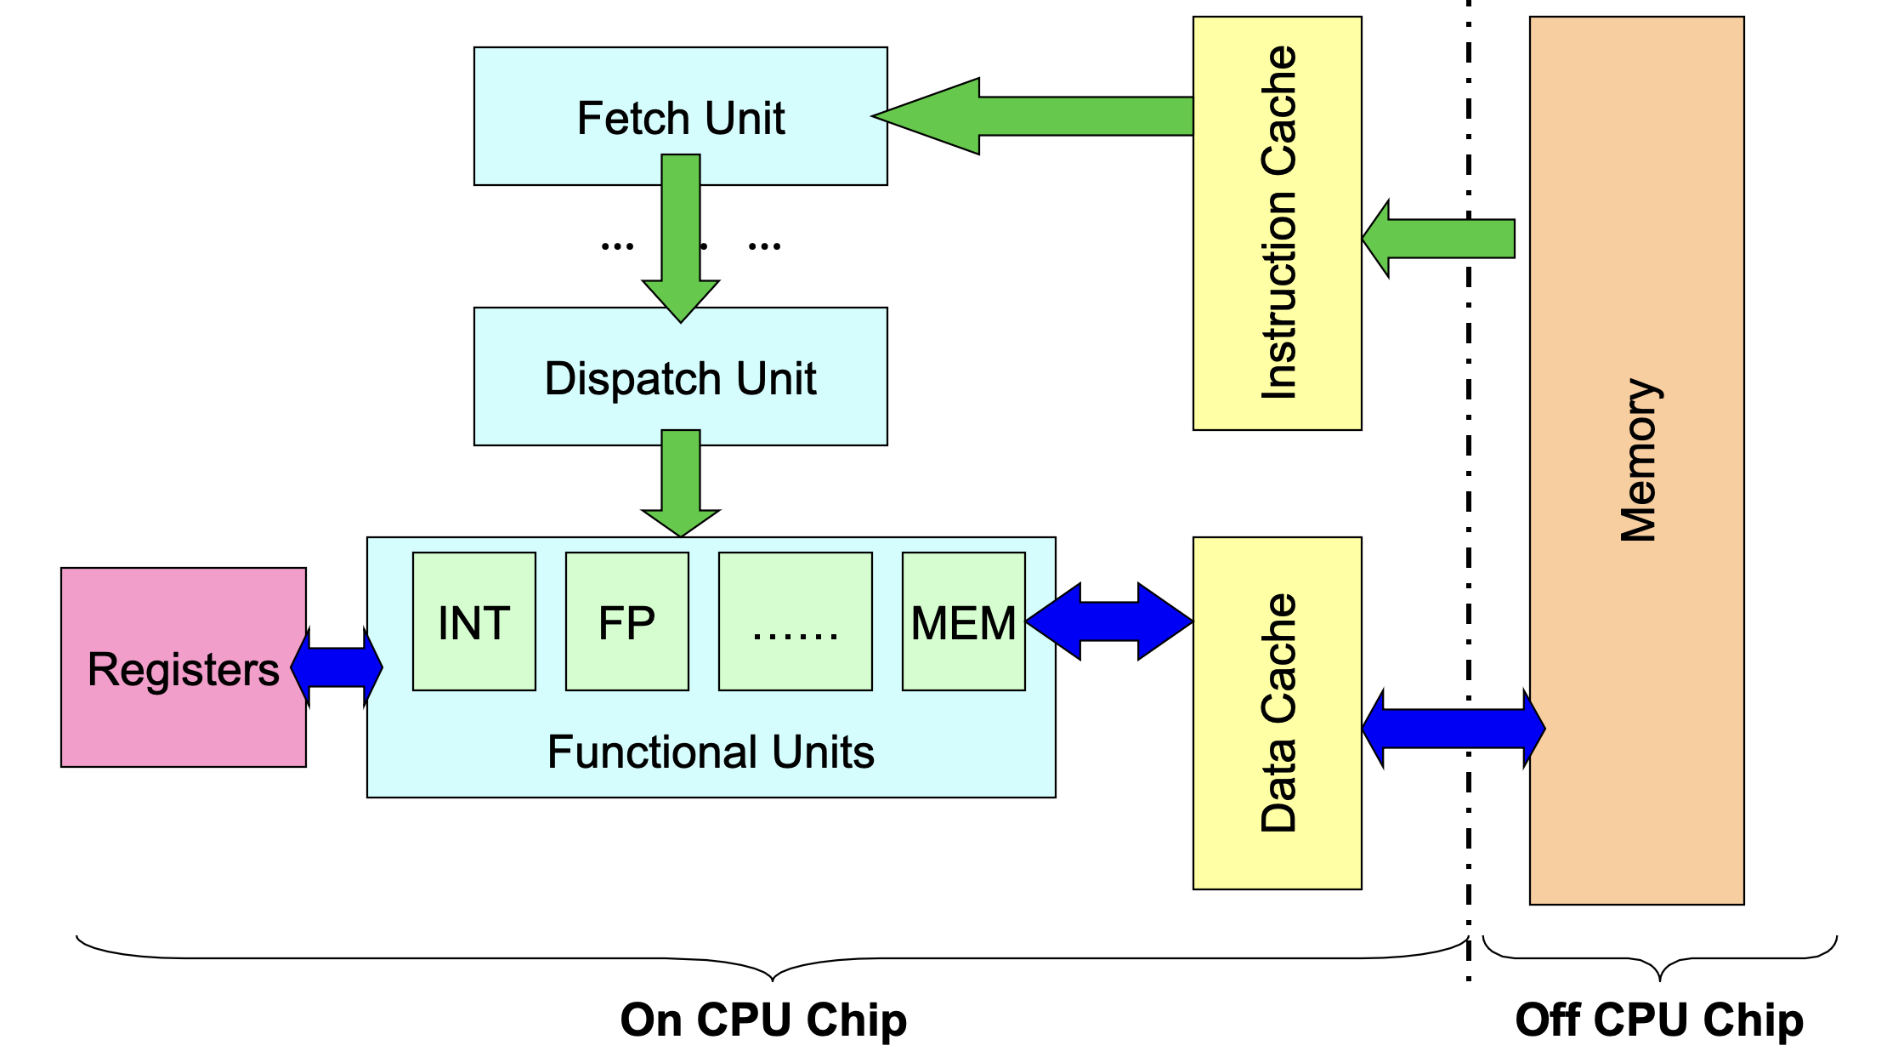
\includegraphics[scale=0.27]{computer-organisation}
\subsubsection{Memory}
\begin{itemize}
	\item Storage for instruction and data
	\item Managed by the OS
	\item Normally accessed via load/store instructions
\end{itemize}
\subsubsection{Cache}
\begin{itemize}
	\item Fast and invisible to software
	\item Duplicate part of the memory for faster access
	\item Usually split into instruction and data cache
\end{itemize}
\subsubsection{Fetch}
\begin{itemize}
	\item Load instructions from memory
	\item Location indicated by \textbf{Program Counter}
\end{itemize}
\subsubsection{Functional units}
\begin{itemize}
	\item Carry out instruction execution
	\item Dedicated to specific instruction type
\end{itemize}
\subsubsection{Registers}
\begin{itemize}
	\item Internal storage for fastest access speed
\end{itemize}

\subsection{Information needed}
\begin{itemize}
	\item Memory context
	\begin{itemize}
		\item Code
		\item Data
	\end{itemize}
	\item Hardware context
	\begin{itemize}
		\item Register
		\item PC value
		\item Frame Pointer
	\end{itemize}
	\item OS context
	\begin{itemize}
		\item Process properties
		\item Resources used
		\item Files
	\end{itemize}
\end{itemize}

\subsection{Function calls}
\subsubsection{Separation of text and data}
Suppose a function f() calls g()
\begin{itemize}
	\item f is caller and g is callee
\end{itemize}
Steps of control flow
\begin{enumerate}
	\item Setup parameters
	\item Trf ctrl to callee
	\item Setup local var
	\item Store any results
	\item Return ctrl to caller
\end{enumerate}
\subsubsection{Issues}
Control Flow
\begin{itemize}
	\item Need to jump to functional body when callee called
	\item Need to resume to next instruction in caller after done
\end{itemize}
Data storage
\begin{itemize}
	\item Need to pass parameters to function
	\item Need to capture return result
	\item May have local variables
\end{itemize}
Additional
\begin{itemize}
	\item May lead to overriding of data in caller by callee (interference)
	\item Calling g() multiple times may lead to insufficient space and overriding
\end{itemize}


\subsection{Stack memory}
Memory to store function invocation
\keyword{Stack Pointer}{Indicates the first free location in the stack region}\\
\keyword{Frame Pointer}{Points to the frame and is used for traversing around the stack easily}\\
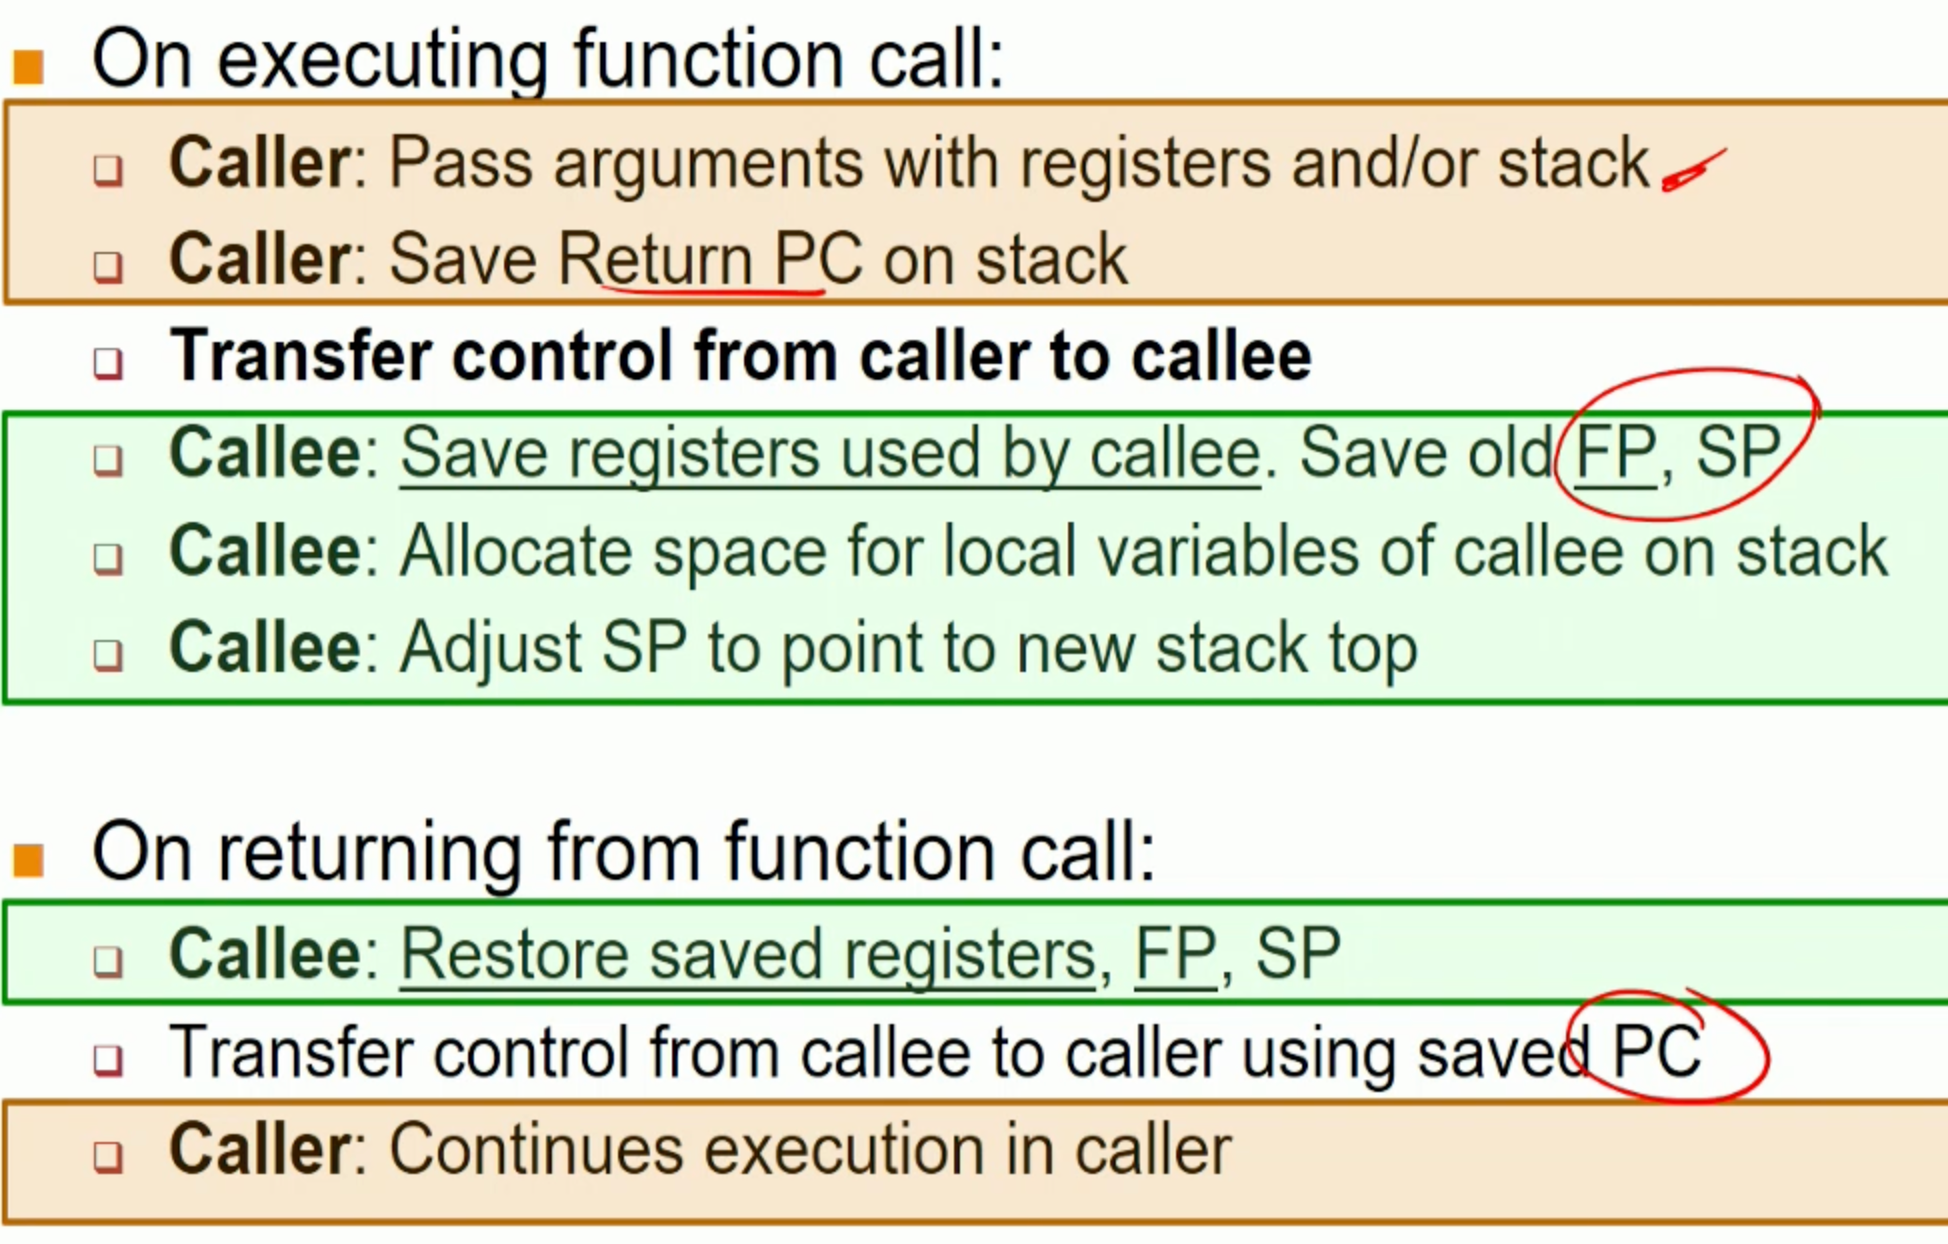
\includegraphics[scale=0.13]{stack-frame}\\
Information needed for function invocation - Stack frame
\begin{itemize}
	\item Return address of caller
	\item Arguments for the function
	\item Local variables
	\item Stack and frame pointer of caller
	\item GPR values (register spilling)
\end{itemize}
Callee stack frame will be on top of the caller


\subsection{Dynamic memory (Heap)}
Memory that the program/user specifies manually (eg. malloc, new)\\
Problems:
\begin{itemize}
	\item Allocated only at runtime
	\begin{itemize}
		\item Size not known at program compilation time
		\item Cannot specify a region in data 
	\end{itemize}
	\item No definite dellocation timing
	\begin{itemize}
		\item Must be freed explicitly by the program
		\item Cannot place in stack region
	\end{itemize}
\end{itemize}
Solution:\\
Add a region "Heap for dynamic allocation\\
Problems with heap memory:
\begin{itemize}
	\item Generation of holes in between data due to variable deallocation timing
\end{itemize}

%-----------------------------------------------------------------------------------------------------------------------
\subsection{OS context}
\subsubsection{Process identification}
Features:
\begin{itemize}
	\item Distinguish processes from each other (Unique)
	\item Communicated to the hardware
\end{itemize}
\subsubsection{Process state}
\begin{itemize}
	\item Denotes whether a process is running or not (Running vs waiting vs not running)
\end{itemize}
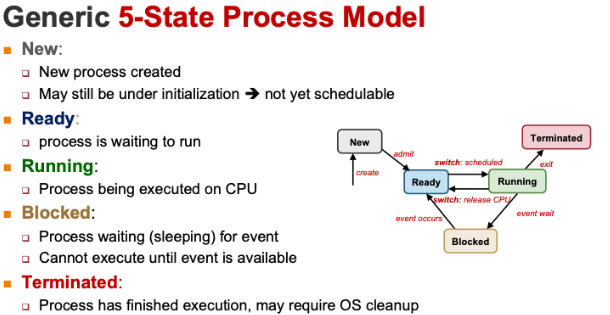
\includegraphics[scale=0.48]{process-model}

\keyword{Process control block}{Table representing all processes}

\subsection{Exceptions and interrupts}
Exceptions
\begin{itemize}
	\item Synchronous (due to program execution)
	\item Machine level instructions arise errors
	\item Exception handler executed automatically in software
\end{itemize}
Interrupts
\begin{itemize}
	\item Asynchronous (Can happen anytime)
	\item External events that cause execution to fail (hardware related errors)
	\item Program execution suspended and \textbf{interrupt handler} executed automatically
\end{itemize}

\subsubsection{Instruction execution}
\begin{enumerate}
	\item Read byte from PC and decode instruction
	\item Read 2 bytes to get the address/operands
	\item Perform ALU operations
	\item Store result into destination
	\item Check if any interruptions
\end{enumerate}
Interrupts can happen at anytime, and will remain pending until step 5 where it is handled

\subsubsection{Interruption handling}
\begin{enumerate}
	\item Push PC and status register into hardware
	\item Disable interrupts
	\item Read \keyword{Interrupt Vector Table}{Table where the OS stores address of all interrupt handlers}
	\item Switch to kernel mode
	\item Set PC to handler address and execute the instructions
\end{enumerate}
\begin{itemize}
	\item OS populates the IVT table with address of interrupt routines
	\item Hardware reads IVT to locate the handler
\end{itemize}

\subsection{System calls}
\keyword{Application Program Interface}{Provides way of calling facilities/services in kernel}\\
Instructions can only be done in kernel mode

\subsubsection{Method}
\begin{itemize}
	\item Library version with the same name and same arguments
	\item User friendly library version
	\item using the function $long~syscall(long~number);$
\end{itemize}
\subsubsection{Mechanism}
\begin{enumerate}
	\item User invoke library call
	\item Place call number in the designated location
	\item Library call executes a special instruction (\textbf{TRAP/syscall}) to change user to kernel mode
	\item (in kernel) syscall handler is determined (by a \textbf{dispatcher})
	\item syscall handler is executed
	\item Syscall handler ends and control returned to the library call
	\item Return to user mode and continue normal function mechanism
\end{enumerate}



%--------------------------------------------------------------------------------------------------------------------
\section{03. Process abstraction in Unix}
Process information
\begin{description}
	\item[Pid]
	\item[Process state]{Running, sleeping, stopped, \keyword{zombie}{Process that has stopped but resources not cleared}}
	\item[Parent pid]
	\item[Cumulative CPU time]{For scheduling}
\end{description}

\subsection{fork()}
Process creation
\begin{description}
	\item[Package]{unistd.h and sys/types.h}
	\item[return]{PID of newly created process(parent) and 0 (child process)}
\end{description}
\subsubsection{Behaviour}
\begin{itemize}
	\item Creates a child process
	\begin{itemize}
		\item \textbf{Copy} data of parent (Independent memory space)
		\item Sane code, same address space
		\item Differs by pid, ppid and fork() return value
	\end{itemize}
\end{itemize}

\subsubsection{Implementation}
Clone the parent process 
\begin{enumerate}
	\item Create address space of child process
	\item allocate new pid to child and pass to parent
	\item Create kernel process data structures
	\item Copy kernel environment of parent process
	\item Initialize child process context (pid, ppid, cpu\_time = 0)
	\item Copy memory regions from parent
	\begin{itemize}
		\item Very expensive operation
		\item Code, data, stack
	\end{itemize}
	\item Acquire shared resources
	\item Initialize hardware context for child process (copy parent registers)
\end{enumerate}

Problem: Memcopy is very expensive operation\\
Solution: Copy on write
\begin{itemize}
	\item Only duplicate a memory location when it is written to
\end{itemize}

\subsection{exec(@param)}
Replace current executing process image
\begin{itemize}
	\item code and data replaced
	\item PID intact
\end{itemize}
Format
\begin{description}
	\item[param]{char *path, char *arg0...}
	\begin{itemize}
		\item Note that last term MUST be \textbf{NULL} indicating end of argument list
	\end{itemize}
	\item[header]{unistd.h}
\end{description}

\subsection{exit(status)}
\begin{description}
	\item[return]{Does not return anything}
	\item[param]{int status - returned to the wait call}
\end{description}
\begin{itemize}
	\item Most system resource used by process are released on exit
	\item return from main() implicitly calls exit(0)
	\item Basic processes are not releasable
	\begin{itemize}
		\item Pid and status
		\item Process accounting info
	\end{itemize}
\end{itemize}

\subsection{wait(\&status)}
Parent child synchronisation
\begin{description}
	\item[param]{\&status - address to put return value}
	\item[header]{sys/types.h and sys/wait.h}
	\item[return]{pid of terminated process}
\end{description}
\begin{itemize}
	\item Call is blocking - suspend operation until at least one child terminates
	\item Cleans up remainder of child system resources (PID, status)
	\item waitpid - used for waiting for specific child process
\end{itemize}

\subsection{Orphan and zombie process}
\keyword{Zombie}{Process that has exited but parent did not call wait}\\
\keyword{Orphan}{Child process whose parent has been terminated}
\begin{itemize}
	\item Parenthood will be propagated up to init which may use wait() to clean up
\end{itemize}


%--------------------------------------------------------------------------------------------------------------------
\section{04. Inter Process Communication}

\subsection{Mechanism}
\begin{itemize}
	\item Shared memory
	\item Message passing
	\begin{itemize}
		\item Pipes
		\item Signal
	\end{itemize}
\end{itemize}

\subsection{Shared memory}
Communication through read/write to shared memory\\
Advantages
\begin{description}
	\item[Efficient]{Only require OS to setup shared region once}
	\item[Ease of use]{Simple reads and write to memory}
	\begin{itemize}
		\item Implicit communication
		\item Can store any type of information
	\end{itemize}
\end{description}
Disadvantages
\begin{description}
	\item[Limited to single machines]{Less efficient over different system}
	\item[Requires synchronization]{Might have data races without synchronisation}
\end{description}
\keyword{Race condition}{System behaviour is dependent on the context/interleaving of process $\rightarrow$ unpredictable outcome}
Steps of usage
\begin{enumerate}
	\item Create/locate a shared memory region M
	\item Attach M to process memory space
	\item Read from/write to M
	\item Detach M from memory space after use
	\item Destroy M
	\begin{itemize}
		\item Only one process need to do this
		\item Can only destroy if M is not attached to any process
	\end{itemize}
\end{enumerate}

\subsection{Message Passing}
Explicit communication through exchange of message
\begin{description}
	\item[Naming]{Have to identify the parties in the communication}
	\item[Synchronisation]{Behaviour of sending/receiving operations}
\end{description}
\begin{itemize}
	\item Messages have to be stored in kernel memory space
	\item All sending/receiving operations have to be done through syscalls
\end{itemize}
\subsubsection{Direct communication}
Sender/receiver explicitly name parties in communication
\begin{itemize}
	\item One link per pair of communicating processes
	\item Need to know identity of other party
\end{itemize}

\subsubsection{Indirect communication}
Messages sent to message storage (\textbf{Mailbox/Port})
\begin{itemize}
	\item Can be shared among a number of processes
\end{itemize}

\subsubsection{Synchronisation behaviour}
Blocking
\begin{itemize}
	\item send and receive is blocked until a message has received/sent (other party is ready)
\end{itemize}
Non-blocking (asynchronous)
\begin{itemize}
	\item execute immediately and sends information to somebody OR returns empty handed
\end{itemize}
Typically, receive is synchronous and send is asynchronous\\
BUT send just buffers the message and only sends the message when the receiver is receiving (no loss)\\
Message buffers
\begin{itemize}
	\item Under OS control 
	\item Decouples sender and receiver -\> less sensitive to variation in execution
	\item Mailbox capacity declaration in advance
\end{itemize}
\textbf{Rendezvous}
\begin{itemize}
	\item Synchronous message passing 
	\item Sender is blocked until receiver sends matching receive
	\item No buffering needed
\end{itemize}

\subsubsection{Pros}
\begin{itemize}
	\item Applicable beyond a single machine
	\item \keyword{Portable}{Easily implemented on many platforms and processing environments}
	\item Easier synchronisation
	\begin{itemize}
		\item Implicit via send/receive behaviour
		\item Communication and synchronisation is done simultaneously
	\end{itemize}
\end{itemize}
\subsubsection{Cons}
\begin{description}
	\item[Inefficient]{Usually requires OS intervention every operation}
	\item[Difficult to use]{Requires information packing into specific format}
\end{description}

\subsection{Unix Pipes}
3 different communication channels to user
\begin{enumerate}
	\item stdin - standard in bounded to keyboard input
	\item stderr - used for error messages
	\item stdout - linked to screen
\end{enumerate}
$"|"$ symbol for linking input/output channels of each process to each other\\
Create communication channel with 2 ends (one reading, one writing)\\
\begin{itemize}
	\item Producer-consumer relationship
	\item Like anonymous file reading information FIFO
\end{itemize}

\subsubsection{Synchronisation}
\begin{itemize}
	\item Circular bounded byte buffer with implicit synchronization
	\item Writer wait when buffer is full
	\item Reader wait when buffer is empty
	\item Unidirectional (one write one read exclusively) vs bidirectional (any end for reading and writing)
\end{itemize}
\subsubsection{pipe(@param)}
\begin{description}
	\item[param]{array of file descriptors}
	\item[return]{0 for success, != for errors}
\end{description}

%--------------------------------------------------------------------------------------------------------------------
\section{05.Synchronisation}
%--------------------------------------------------------------------------------------------------------------------
\section{06.Synchronisation primitives}
%--------------------------------------------------------------------------------------------------------------------
\section{07.Threads}
\subsection{Motivation}
\begin{itemize}
	\item Processes are expensive
	\begin{itemize}
		\item Process creation via fork() duplicates memory space and process context
		\item Requires context switching and saving/restoring process information repeatedly
	\end{itemize}
	\item Hard to communicate with each other
	\begin{itemize}
		\item Independent memory space (IPC communication only)
	\end{itemize}
	\item Need easy way to execute some instructions simultaneously (more threads of control to same process)
\end{itemize}
\subsection{Features}
\begin{itemize}
	\item \keyword{Multithreaded process}{Single process with multiple threads}
	\item Threads share the same \textbf{Memory context}(Text, data, heap) and \textbf{OS context}(PID)
	\item Contains unique information
	\begin{itemize}
		\item Identification (thread id)
		\item Registers (GPR and special)
		\item Stack
	\end{itemize}
\end{itemize}

\subsection{Benefits}
\begin{description}
	\item[Economy]{Less resources to manage}
	\item[Resource sharing]
	\item[Responsiveness]
	\item[Scalability]{Can take advantage of multiple CPUs}	
\end{description}

\subsection{Problems}
\begin{itemize}
	\item Syscall concurrency
	\begin{itemize}
		\item Parallel execution of threads may result in parallel syscalls
	\end{itemize}
	\item Process behaviour
	\begin{itemize}
		\item Unable to impact process operations
	\end{itemize}
\end{itemize}

\subsection{Thread implementation}
\begin{enumerate}
	\item User thread
	\begin{itemize}
		\item Implemented as a user library -\> More flexible and configurable
		\item Runs on any OS
		\item Kernel unaware of threads in process (scheduling at process level)
	\end{itemize}
	\item Kernel thread
	\begin{itemize}
		\item Implemented in the OS through syscalls (slower and more resource intensive)
		\item Scheduling among threads instead of via process
		\item Use threads in kernel operations
		\item Less flexible
		\begin{itemize}
			\item Used by all multithreaded programs so kernel must cater to all
			\item Balance btw many and less features
		\end{itemize}
	\end{itemize}
	\item Hybrid thread
	\begin{itemize}
		\item OS schedules on kernel threads
		\item User threads can be bound to kernel threads
		\item Lead to greater flexibility
	\end{itemize}
\end{enumerate}

\subsection{Posix Threads (pthreads)}
\subsubsection{pthread\_create}
\begin{description}
	\item[param]{tid, attributes, \&function, function\_params}
	\item[return]{0 success, != 0 fail}
\end{description}

\subsubsection{pthread\_exit}
\begin{description}
	\item Automatically called after function finishes
	\item[param]{exit\_value}
	\item[behaviour]{return value of function will be the "exit value"}
\end{description}

\subsubsection{pthread\_join}
\begin{description}
	\item[param]{tid, \keyword{\&status}Exit value returned by target pthread}
\end{description}

%--------------------------------------------------------------------------------------------------------------------
\section{08.Synchronization classics}
\end{multicols*}
\end{document}